\section{Sequence diagrams}

\subsection{Introduction}

\begin{flushleft}
Les sequences diagrams nous permettent de détailler le chemin effectué lorsqu'un utilisateur souhaite intéragir avec l'application.
\end{flushleft}

\begin{flushleft}
Dans le but de permettre une meilleure compréhension de ces diagrammes, nous les avons séparés en trois parties.
\begin{enumerate}
\item Common
\item Client
\item Provider
\end{enumerate}
\end{flushleft}

\begin{flushleft}
Afin de les réaliser convenablement, nous sommes repartis de notre class diagram et nos Use cases diagrams et avons représenté l'interaction des méthodes avec l'API et la base de données.
\end{flushleft}

\begin{flushleft}
Avant de commencer, il est important de signaler dans le but d'éviter toute répétition, que la vérification du token s'effectuera pour chaque action lorsqu'un utilisateur est connecté.
\end{flushleft}

\begin{flushleft}
Si le token est bon, on continue le programme, sinon, on envoie un message d'erreur à l'aide de la méthode "sendMessageError".
\end{flushleft}

\begin{flushleft}
Pour rappel, l'utilisateur n'appelle pas directement les méthodes partant de sa lifeline mais utilise des requêtes de l'API. De plus, vous pouvez constater que dans le diagramme des classes, nous n'avons pas mis de type de retour aux méthodes de l'API. Cependant, dans les diagrammes de séquences, nous avons quand-même représenté une flèche de retour. Cela est dû au fait que pour retourner quelque chose à l'utilisateur, nous utilisons une méthode de la variable routingContext.
\end{flushleft}

\newpage
\subsection{Common}

\begin{flushleft}
Pour la partie commune aux clients et fournisseurs, nous retrouvons plusieurs Use Cases à décrire.
\end{flushleft}

\begin{enumerate}
\item Gérer les données
\item Gérer les langues
\item Modifier son mot de passe
\item Répondre aux notifications
\item S'authentifier
\item Visualisation des données de consommations
\item Voir les contrats
\item Voir notifications
\end{enumerate}

\newpage
\subsubsection{Gérer les données}

\begin{flushleft}
Nous pouvons gérer les données de deux manières. L'utilisateur peut ajouter une donnée de consommation ou en changer une.
\end{flushleft}

\begin{flushleft}
Pour ajouter une donnée, il suffit d'appeler la méthode addConsumption. Cette dernière peut écraser des données selon les paramètres utilisés. Lorsque des données sont écrasées, nous devons donc créer une notification pour prévenir l'autre utilisateur concerné par ce changement.
\end{flushleft}

\begin{flushleft}
Pour changer une donnée, il suffit d'appeler la méthode changeConsumption. Celle-ci change automatiquement une donnée, nous devons donc créer une notification pour prévenir l'autre utilisateur.
\end{flushleft}

\begin{figure}[h]
\centering
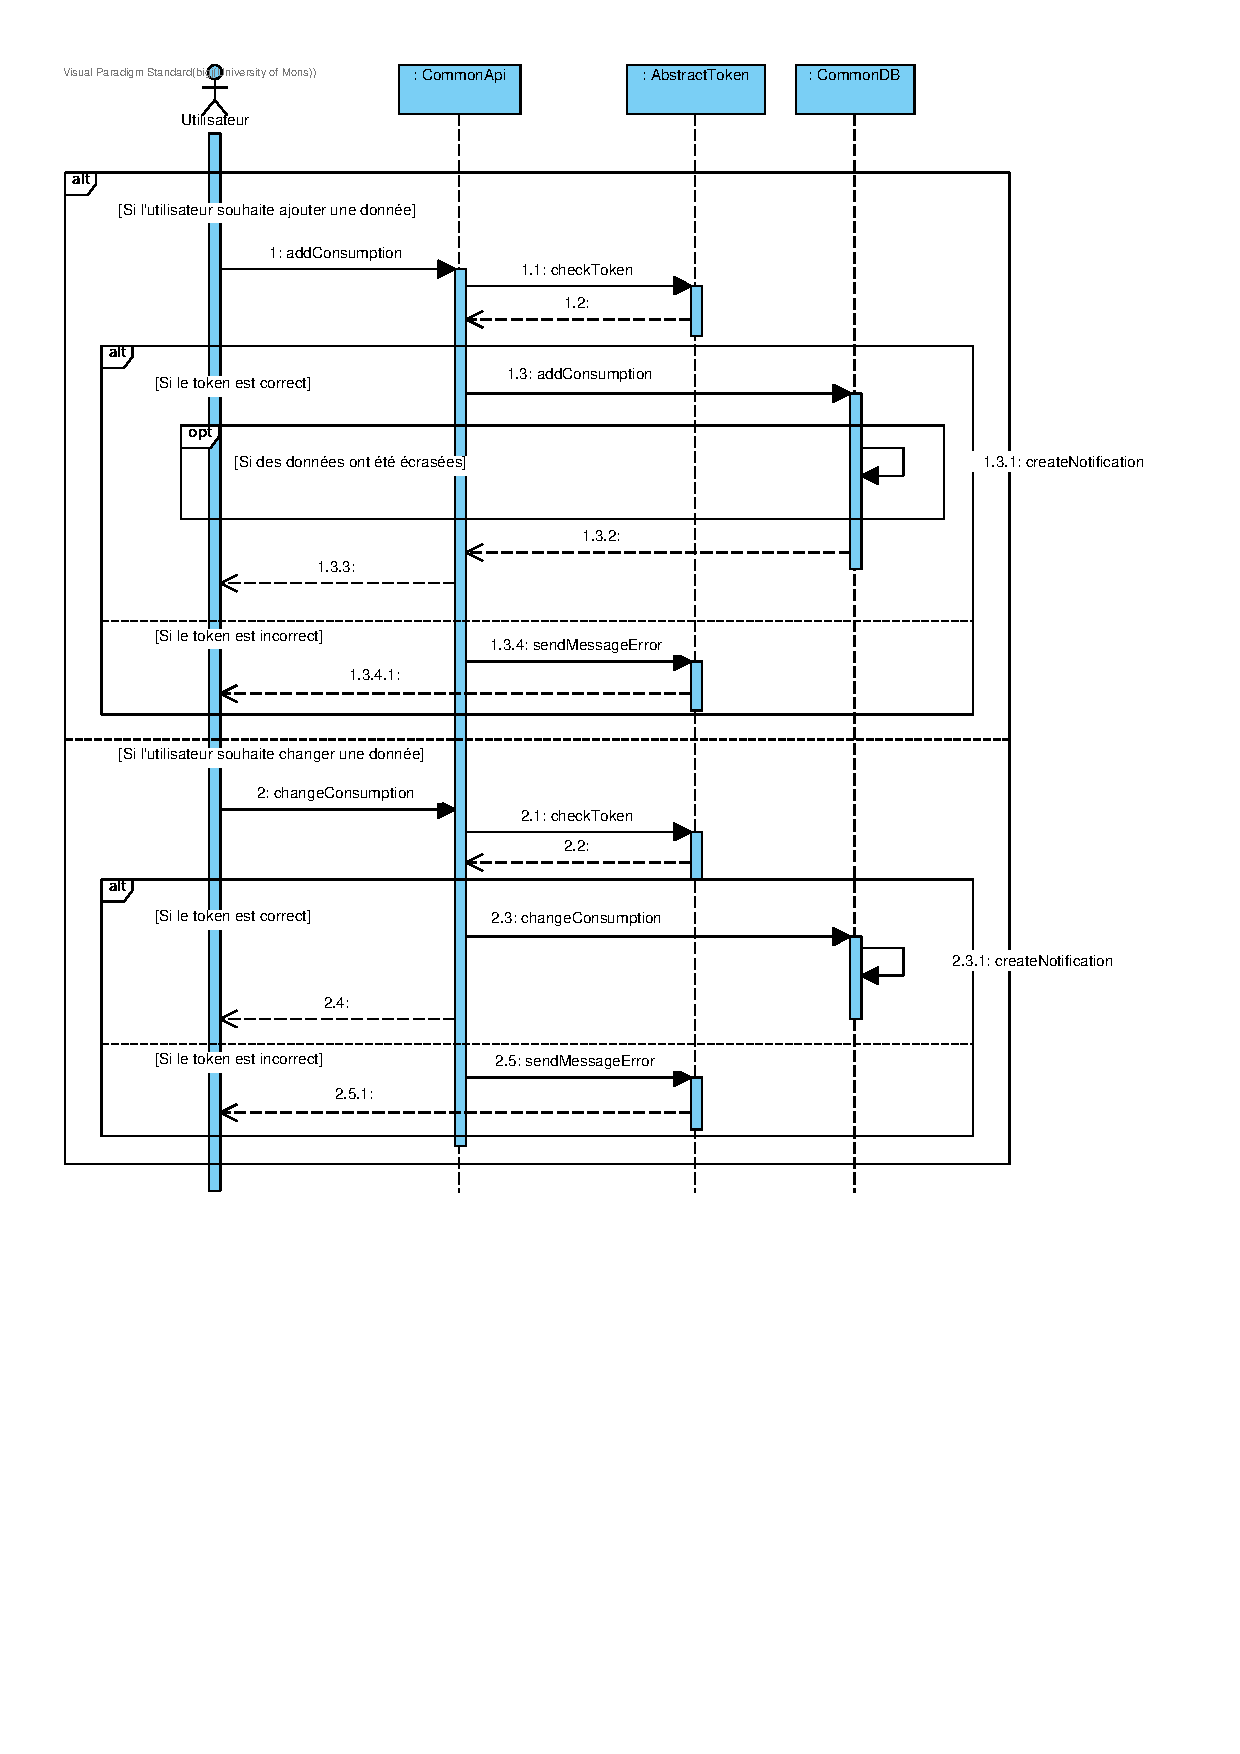
\includegraphics[width = 0.7\textwidth]{Base/sequence/img/common/gerer_les_donne.pdf}
\end{figure}

\newpage
\subsubsection{Gérer les langues}

\begin{flushleft}
Nous pouvons gérer les langues à plusieurs niveaux. L'utilisateur peut voir toutes ses langues, sa langue actuelle et sa langue préférée. En plus de cela, il peut ajouter une langue, changer sa langue actuelle ou encore changer sa langue favorite.
\end{flushleft}

\begin{flushleft}
Pour les trois premières fonctionnalités, le principe est le même. On appelle la méthode adéquate et celle-ci va t'être rappelée dans la partie base de donnée pour rechercher l'information désirée.
\end{flushleft}

\begin{flushleft}
Concernant les autres fonctionnalités, on appelle également la méthode du même nom dans la partie base de données. Remarquez que ces méthodes ne retournent rien.
\end{flushleft}

\begin{figure}[h]
\centering
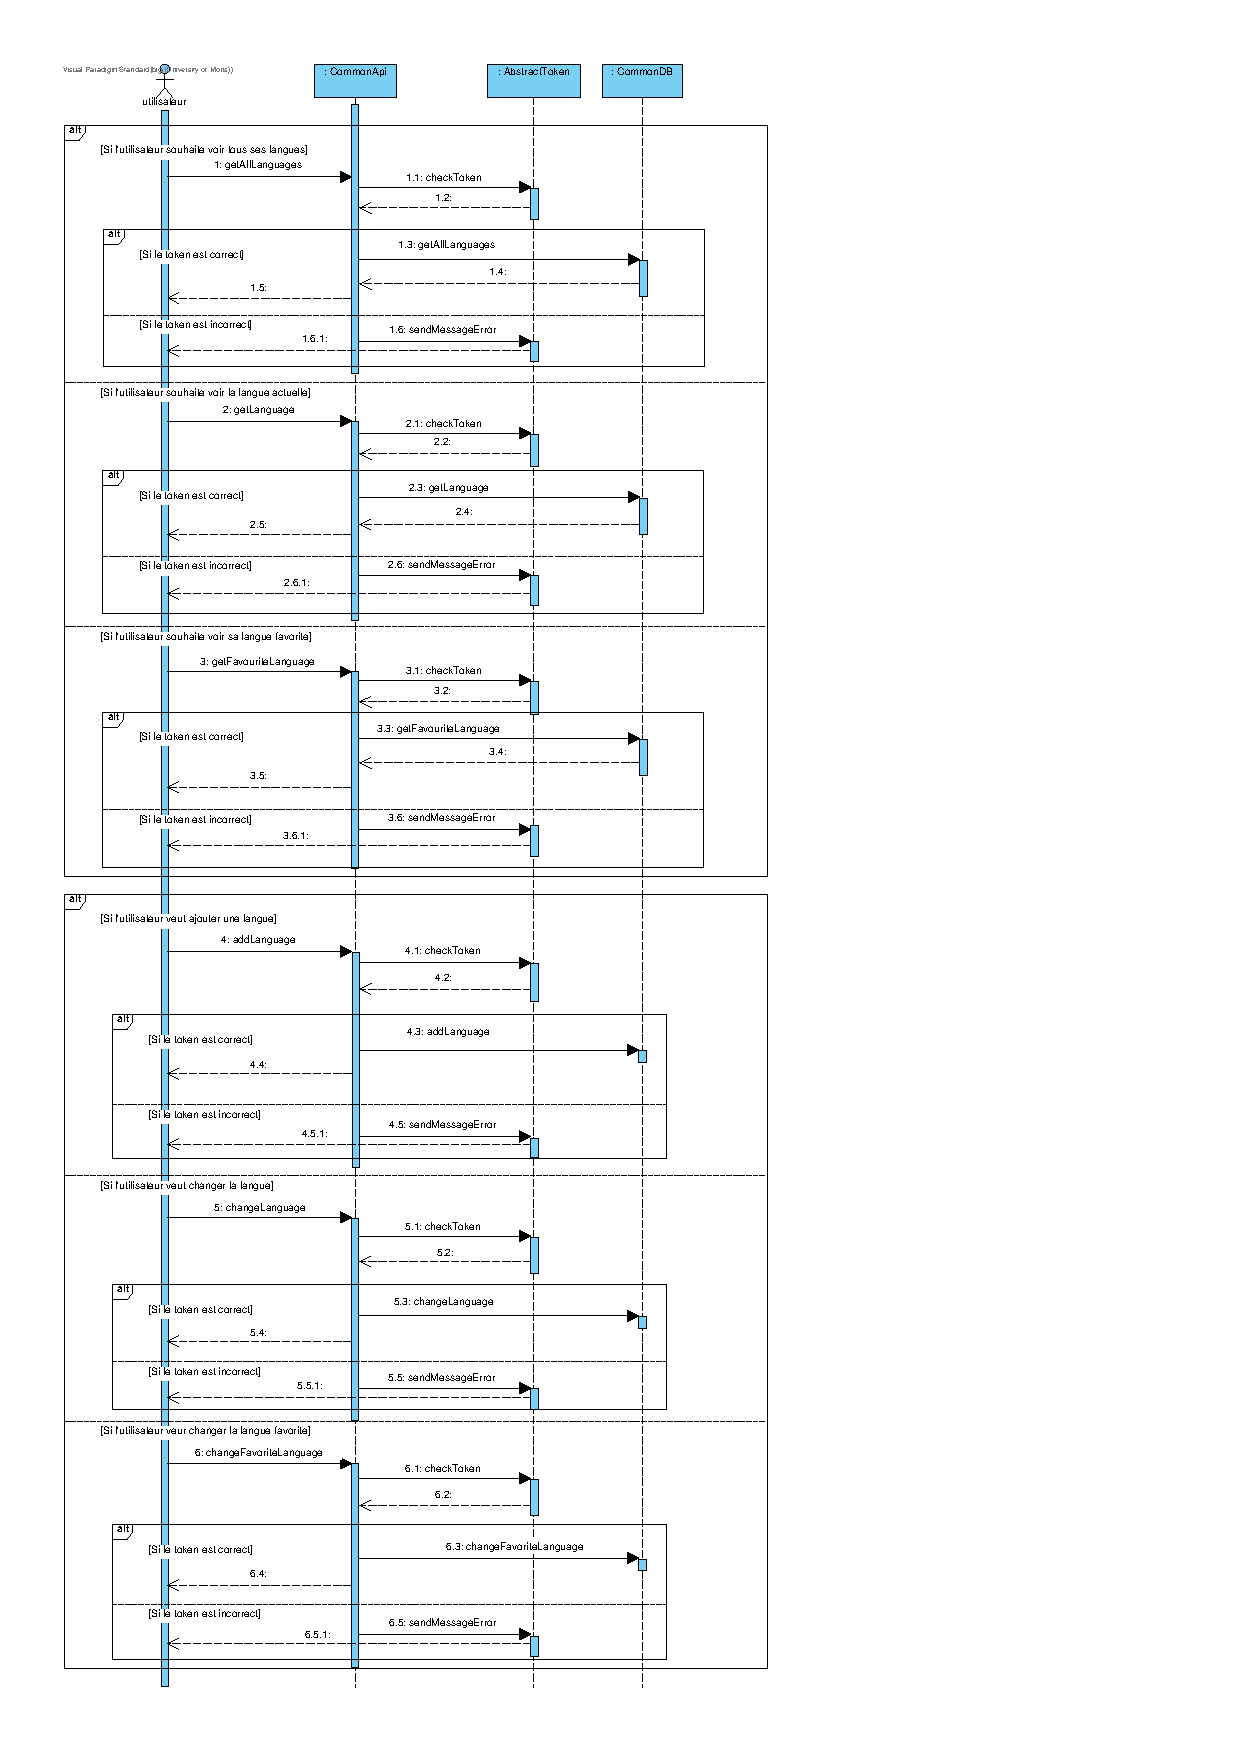
\includegraphics[height = 1\textwidth]{Base/sequence/img/common/gerer_les_langues.pdf}
\end{figure}

\newpage
\subsubsection{Modifier son mot de passe}

\begin{flushleft}
Pour modifier son mot de passe de manière sécurisée, nous passons par l'adresse mail de l'utilisateur pour être certains que ce soit bien celui-ci qui veuille changer le mot de passe. Pour se faire, il faut tout d'abord faire appel à la méthode getCode, cette dernière va appeler les méthodes createCode et sendEmail de la classe App.
\end{flushleft}

\begin{flushleft}
À noter que createCode va appeler automaticDeleteCode afin que le code se supprime automatiquement au bout d'un laps de temps au cas où l'utilisateur prendrait trop de temps ou n'utiliserait jamais ce code.
\end{flushleft}

\begin{flushleft}
L'utilisateur recevra donc par mail un code de vérification. Il pourra ensuite entrer le code et son nouveau mot de passe sur le site pour finalement appeler la méthode changePwd de l'API. Avant de le changer, nous utilisons la méthode checkCode d'App pour vérifier que le code est correct. Si c'est bien le cas, alors nous pouvons appeler changePwd de CommonDB pour changer le mot de passe. Dans le cas contraire, nous renvoyons évidemment un message d'erreur.
\end{flushleft}

\begin{figure}[h]
\centering
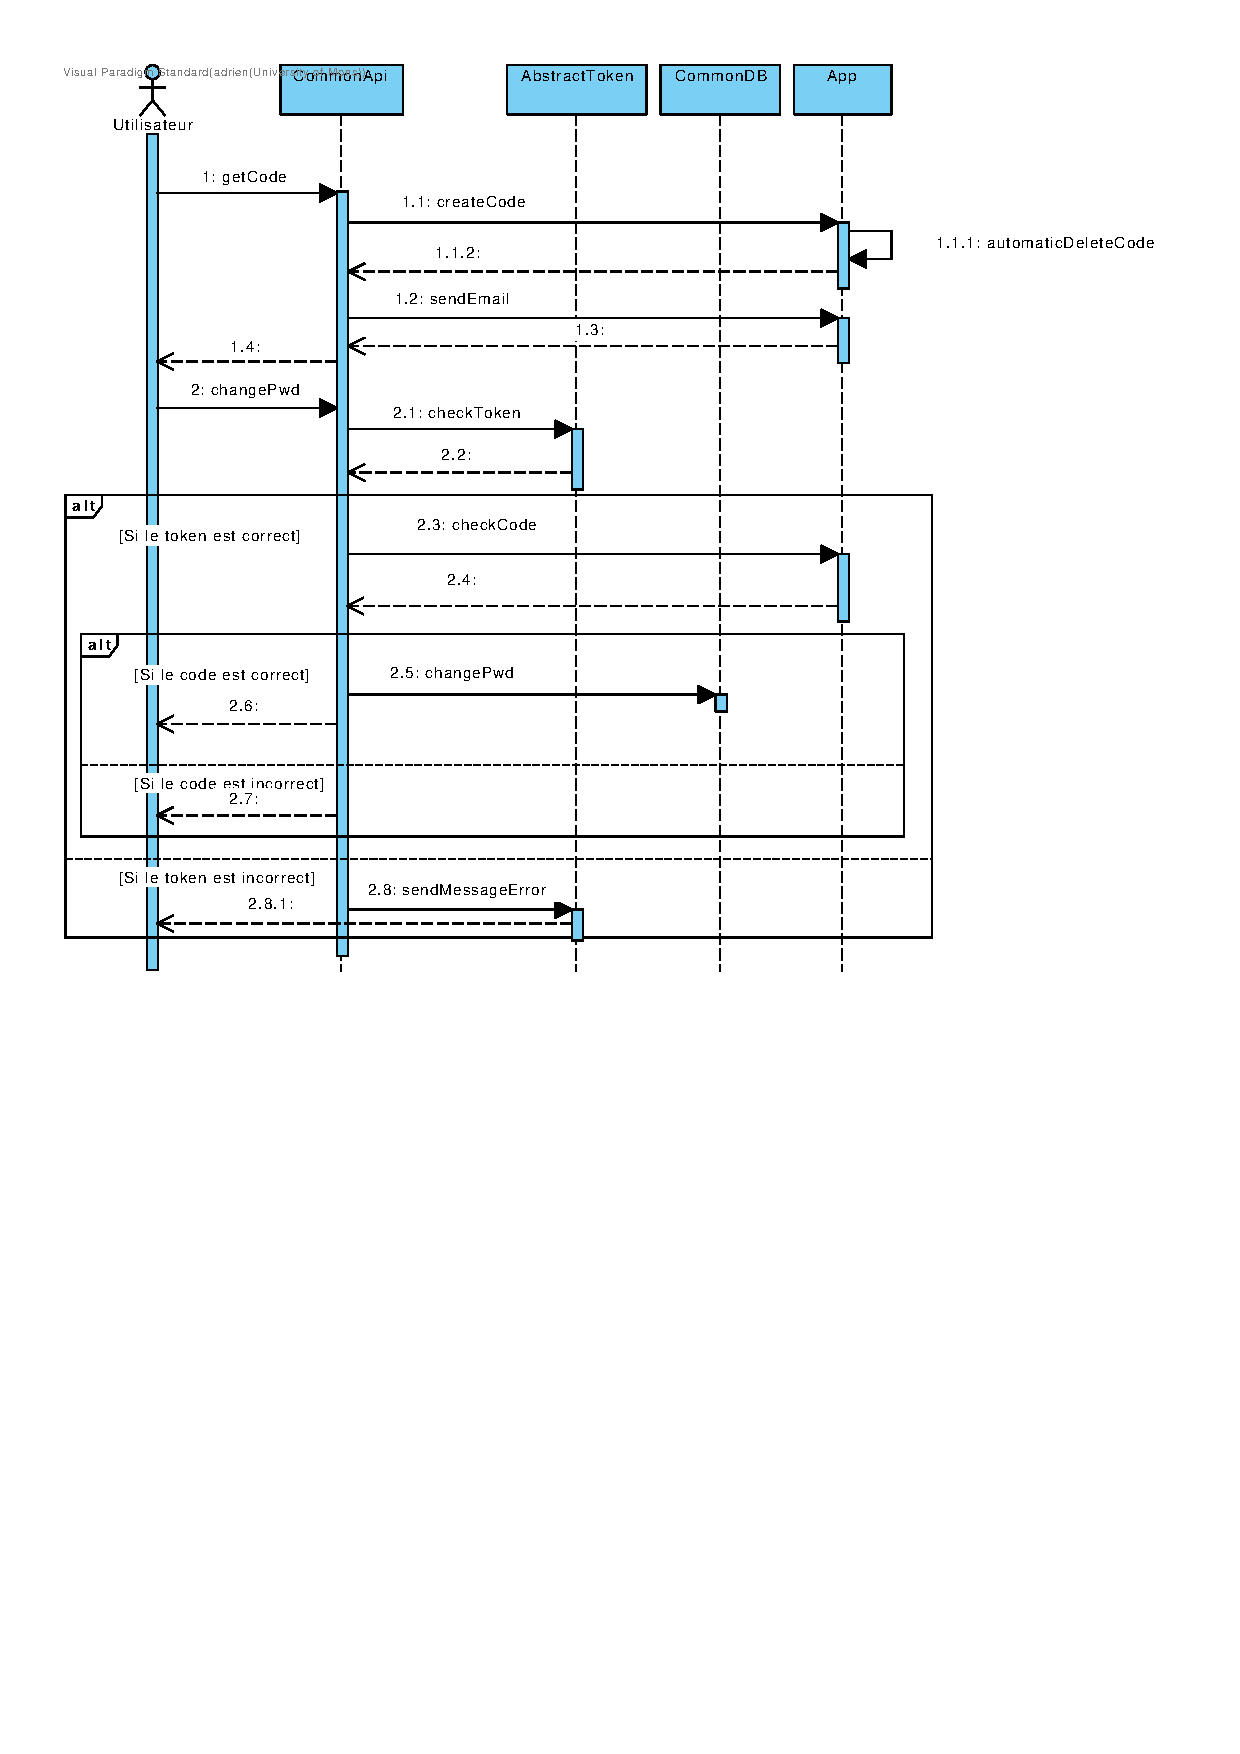
\includegraphics[height = 0.9\textwidth]{Base/sequence/img/common/Modifier son mot de passe.pdf}
\end{figure}

\newpage
\subsubsection{Répondre aux notifications}

\begin{flushleft}
Répondre aux notifications implique trois possibilités. L'utilisateur peut l'accepter ou la refuser dans le cas d'une demande de contrat ou bien dans les autres cas, noter la notification comme lue.
\end{flushleft}

\begin{flushleft}
Lorsqu'un utilisateur accepte une notification (une demande de contrat). Dans la partie base de données, nous commençons par créer un objet contractFull à partir de la proposition acceptée, ensuite nous faisons appel à la méthode createContract pour enregistrer le contrat. Nous pouvons donc supprimer la notification actuelle étant donné qu'elle vient d'être acceptée. Pour finir, nous créons une nouvelle notification pour informer à l'autre utilisateur que sa demande a été acceptée.
\end{flushleft}

\begin{flushleft}
Dans le cas d'une notification informative, l'utilisateur peut la marquer comme lue. Ce qui implique de la supprimer en appelant la méthode deleteNotification.
\end{flushleft}

\begin{figure}[h]
\centering
\includegraphics[height = 0.9\textwidth]{Base/sequence/img/common/répondre_aux_notifications.pdf}
\end{figure}

\newpage

\subsubsection{S'authentifier}

\begin{flushleft}
Lorsque l'utilisateur arrive sur la fenêtre de connexion. Deux cas de base sont possibles. Si l'utilisateur n'a pas de compte ou au contraire s'il en possède déjà un.
\end{flushleft}

\begin{flushleft}
Pour créer un compte, suivant le même principe que le changement de mot de passe. Un code va être crée et envoyé à l'adresse mail que l'utilisateur vient d'entrer grâce aux méthodes déjà expliquées ci-dessus. Quand l'utilisateur souhaite sauvegarder son compte, la méthode saveAcccount est invoquée. Après vérification du code, cette dernière est ré-appelée dans CommonDB pour sauvegarder le compte.
\newline
Suite à cela, Nous pouvons créer un token de connexion grâce à la méthode createToken de la classe abstraite AbstractToken et l'envoyer à l'utilisateur pour ses prochaines requêtes car en créant son compte, il s'est également connecté. Notez que lors de la création du token, nous appelons automaticDeleteToken pour limiter la durée de vie du token.
\end{flushleft}

\begin{flushleft}
Si l'utilisateur possède déjà un compte, nous vérifions les données de connexion grâce à checkAccount. Si les données sont correctes, nous pouvons créer un token et l'envoyer comme expliqué précédemment.
\end{flushleft}

\begin{flushleft}
Si l'utilisateur possède un compte mais ne parvient pas à se connecter. Il a la possibilité de réinitialiser son mot de passe. Le processus utilisé est le même que lors du changement de mot de passe expliqué précédemment.
\end{flushleft}

\begin{flushleft}
Une fois connecté, l'utilisateur peut de toute évidence se déconnecter en faisant appel à la méthode disconnect. Celle-ci servant juste à appeler deleteToken pour supprimer le token.
\end{flushleft}

\newpage
\begin{figure}[h]
\centering
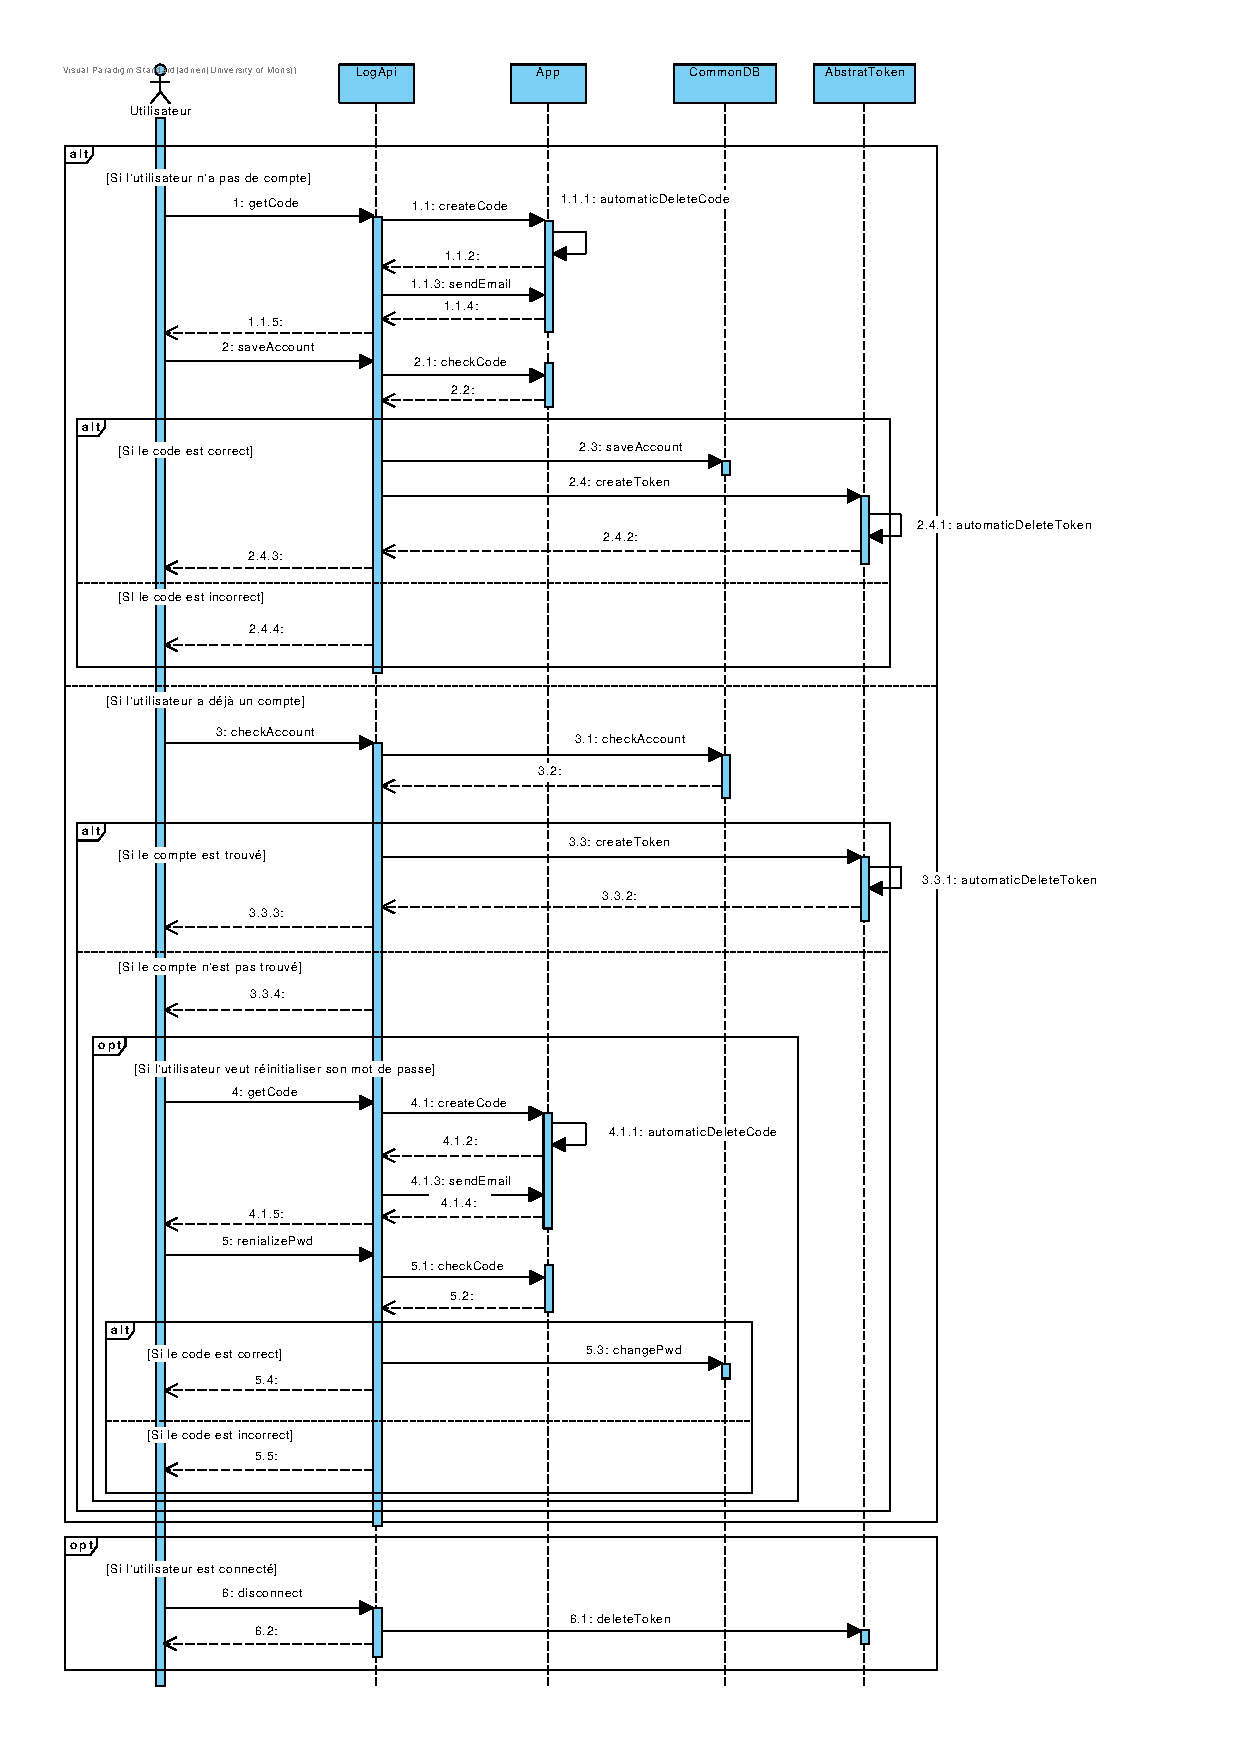
\includegraphics[height = 1\textwidth]{Base/sequence/img/common/S'authentifier.pdf}
\end{figure}

\newpage
\subsubsection{Visualisation des données de consommations}

\begin{flushleft}
Rien de plus simple. Nous invoquons la méthode getConsumption de l'API, ensuite elle est ré-appelée dans CommonDB pour récupérer les valeurs dans la base de données pour finalement les renvoyer.
\end{flushleft}

\begin{figure}[h]
\centering
\includegraphics[height = 1\textwidth]{Base/sequence/img/common/Visualisation des données de consommations.pdf}
\end{figure}

\newpage

\subsubsection{Voir les contrats}

\begin{flushleft}
Au niveau des contrats dans la partie commune, il est possible de voir un contrat en particulier ainsi que d'en supprimer un.
\end{flushleft}

\begin{flushleft}
Il suffit d'appeler la méthode getContract jusqu'à la base de données, nous pouvons ensuite créer un objet ContractFull pour facilement renvoyer les valeurs liées à cet objet. Notez qu'une fois envoyé, l'objet est détruit.
\end{flushleft}

\begin{flushleft}
Comme son nom l'indique, deleteContract permet de supprimer un contrat. Une fois son devoir accompli, cette méthode doit également créer une notification pour avertir l'autre utilisateur impliqué par cette suppression. Il n'est pas utile que cette méthode renvoie quelque chose.
\end{flushleft}

\begin{figure}[h]
\centering
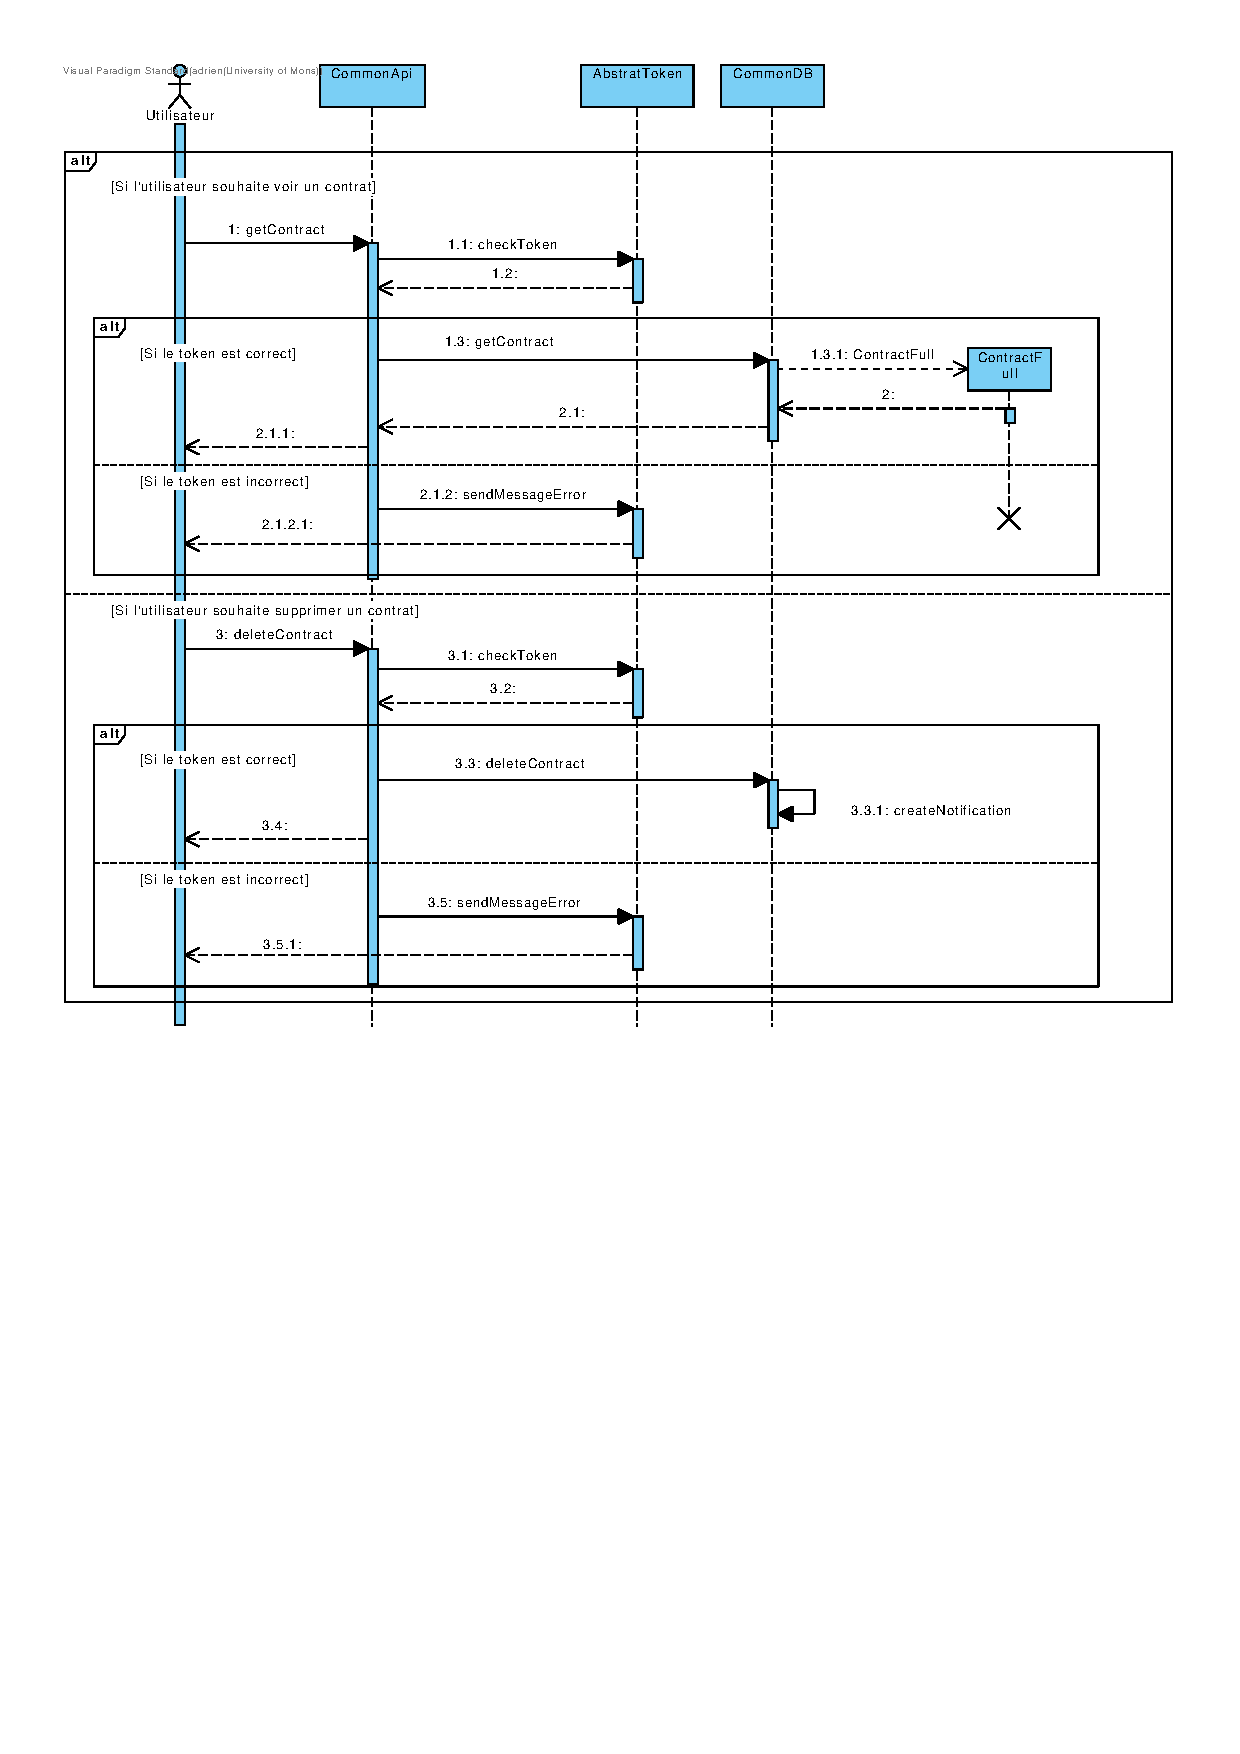
\includegraphics[height = 1\textwidth]{Base/sequence/img/common/Voir les contrats.pdf}
\end{figure}

\newpage

\subsubsection{Voir notifications}

\begin{flushleft}
Pour finir, l'utilisateur peut voir ses notifications. Pour cela, nous suivons toujours le même principe en appelant d'abord la méthode getAllNotifications au niveau de l'API et ensuite dans la partie base de données. Nous créons un objet Notification pour chaque notification stockée pour les envoyer dans une liste vers l'utilisateur. Tous les objets précédemment créés seront évidement supprimés à la suite de l'envoi de la liste.
\end{flushleft}

\begin{flushleft}
Notez que lorsque l'utilisateur rafraîchit les notifications, c'est cette même méthode qui est appelée.
\end{flushleft}

\begin{figure}[h]
\centering
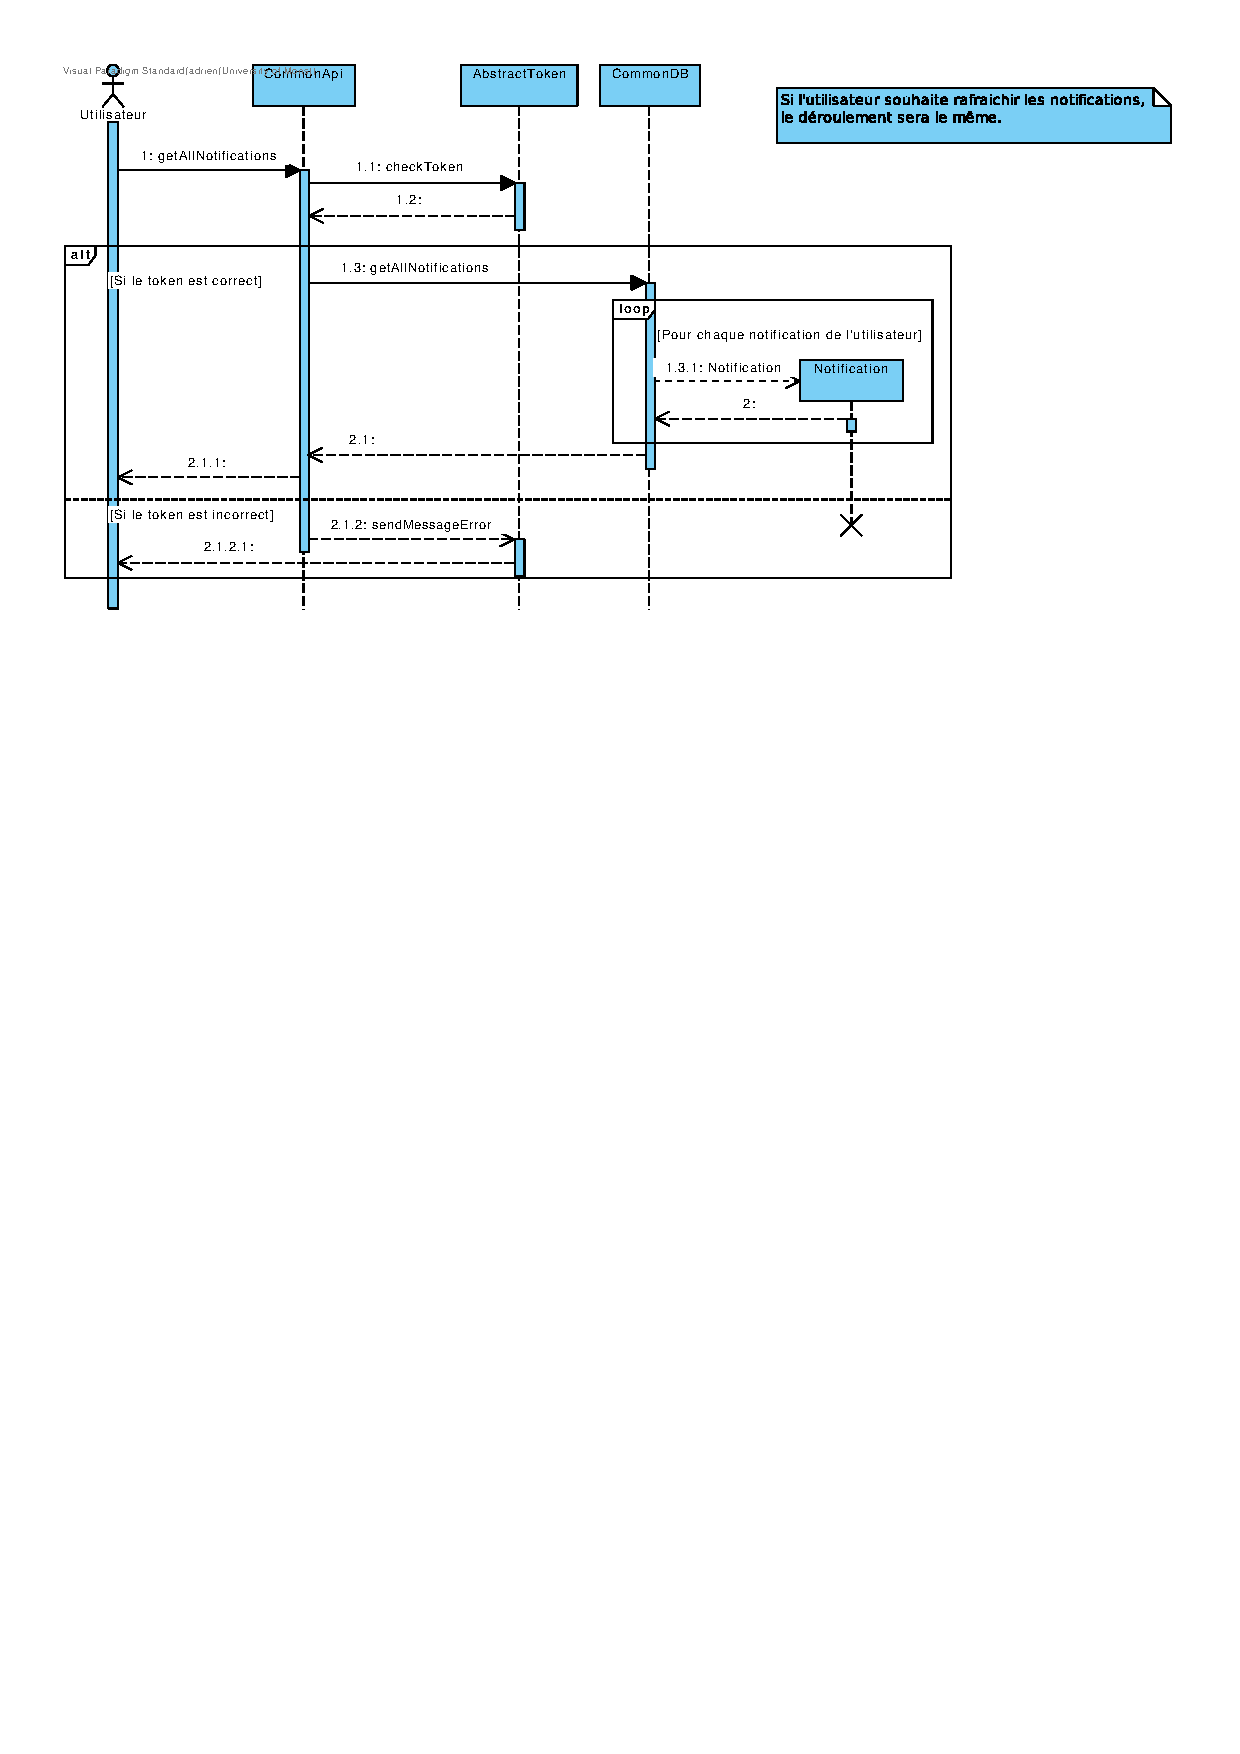
\includegraphics[height = 1\textwidth]{Base/sequence/img/common/Voir notifications.pdf}
\end{figure}

\newpage
\subsection{Client}

\subsubsection{Contrats}\label{CONTRATS}

\begin{flushleft}
Commençons par le Use Case \textbf{"Voir les contrats"}, nous appelons la méthode "getAllContract" de clientApi et ensuite, la méthode du même nom de ClientDB.
\end{flushleft}

\begin{flushleft}
Le but étant d'obtenir une ArrayList de "contractBasic", nous devons effecter une boucle afin de récupérer tous les "contractBasic".
\end{flushleft}

\begin{flushleft}
Une fois effectuée, nous renvoyons cette liste.
\end{flushleft}

\begin{figure}[h]
\centering
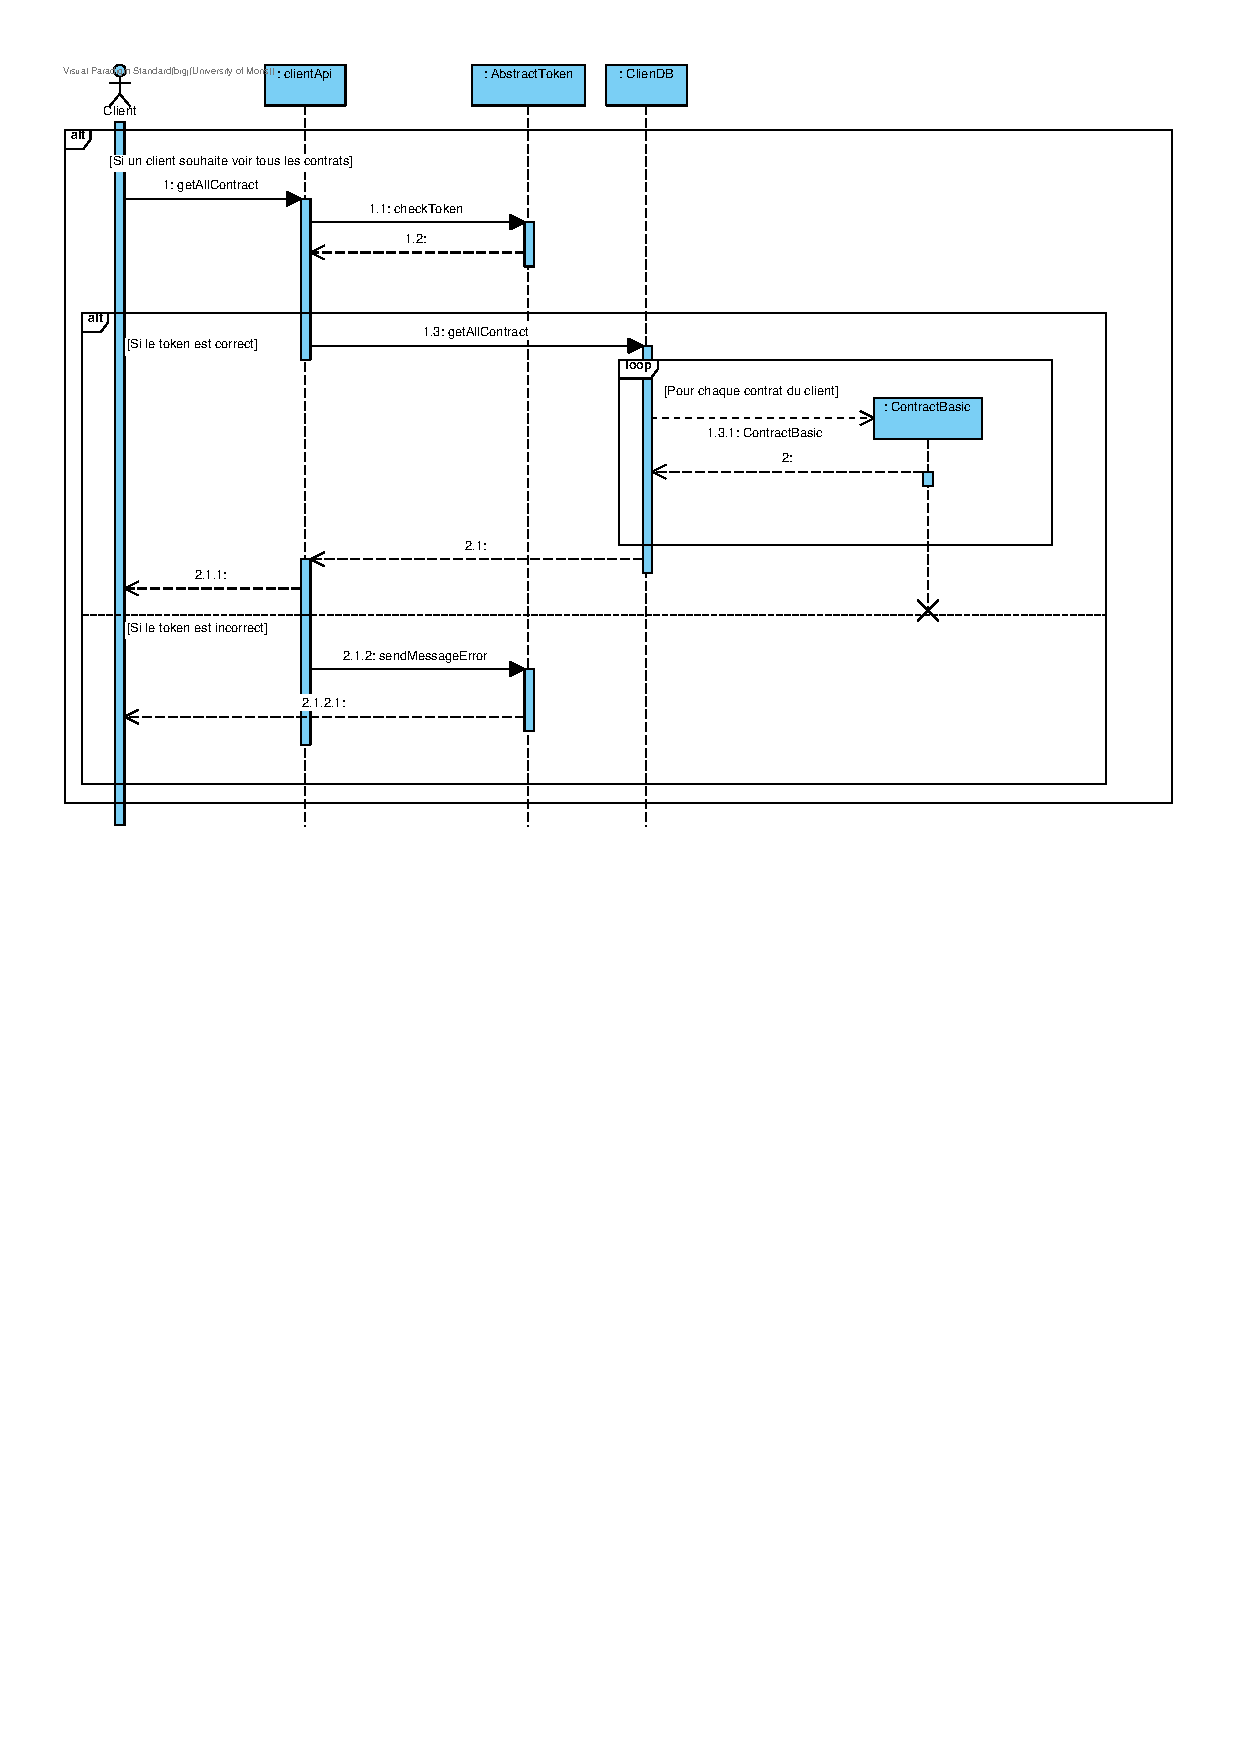
\includegraphics[height = 0.9\textwidth]{Base/sequence/img/client/seqContrats.pdf}
\end{figure}

\newpage

\subsubsection{Fournisseurs et
contrats relatifs}
\begin{flushleft}
Continuons avec l'Use Case \textbf{"Voir les fournisseurs et
contrats relatifs"}.
A cet effet, il y aura deux méthodes :
\end{flushleft}

\begin{enumerate}
\item getAllProposal si le client souhaite voir toutes les propositions.
\item getProposal si le client souhaite voir une proposition en particulier.
\end{enumerate}

\begin{flushleft}
Ces deux méthodes sont appelées une fois de clientApi et ensuite, une fois de ClientDB.
\end{flushleft}

\begin{flushleft}
Dans le cas de "getAllProposal", la valeur de retour est une ArrayList de "proposalBasic" donc nous utiliserons une boucle et dans le cas de "getProposal", nous devons simplement retourner une instance de "proposalFull".
\end{flushleft}

\begin{flushleft}
Concernant le Use Case \textbf{"Ajouter des contrats"}, nous appelons la méthode "clientProposeContract" de clientApi et ensuite, la méthode du même nom de ClientDB.
\end{flushleft}

\begin{flushleft}
Etant donné que cette dernière ne doit rien retourner, il n'y aura pas de valeur de retour.
\end{flushleft}

\newpage
\begin{figure}[h]
\centering
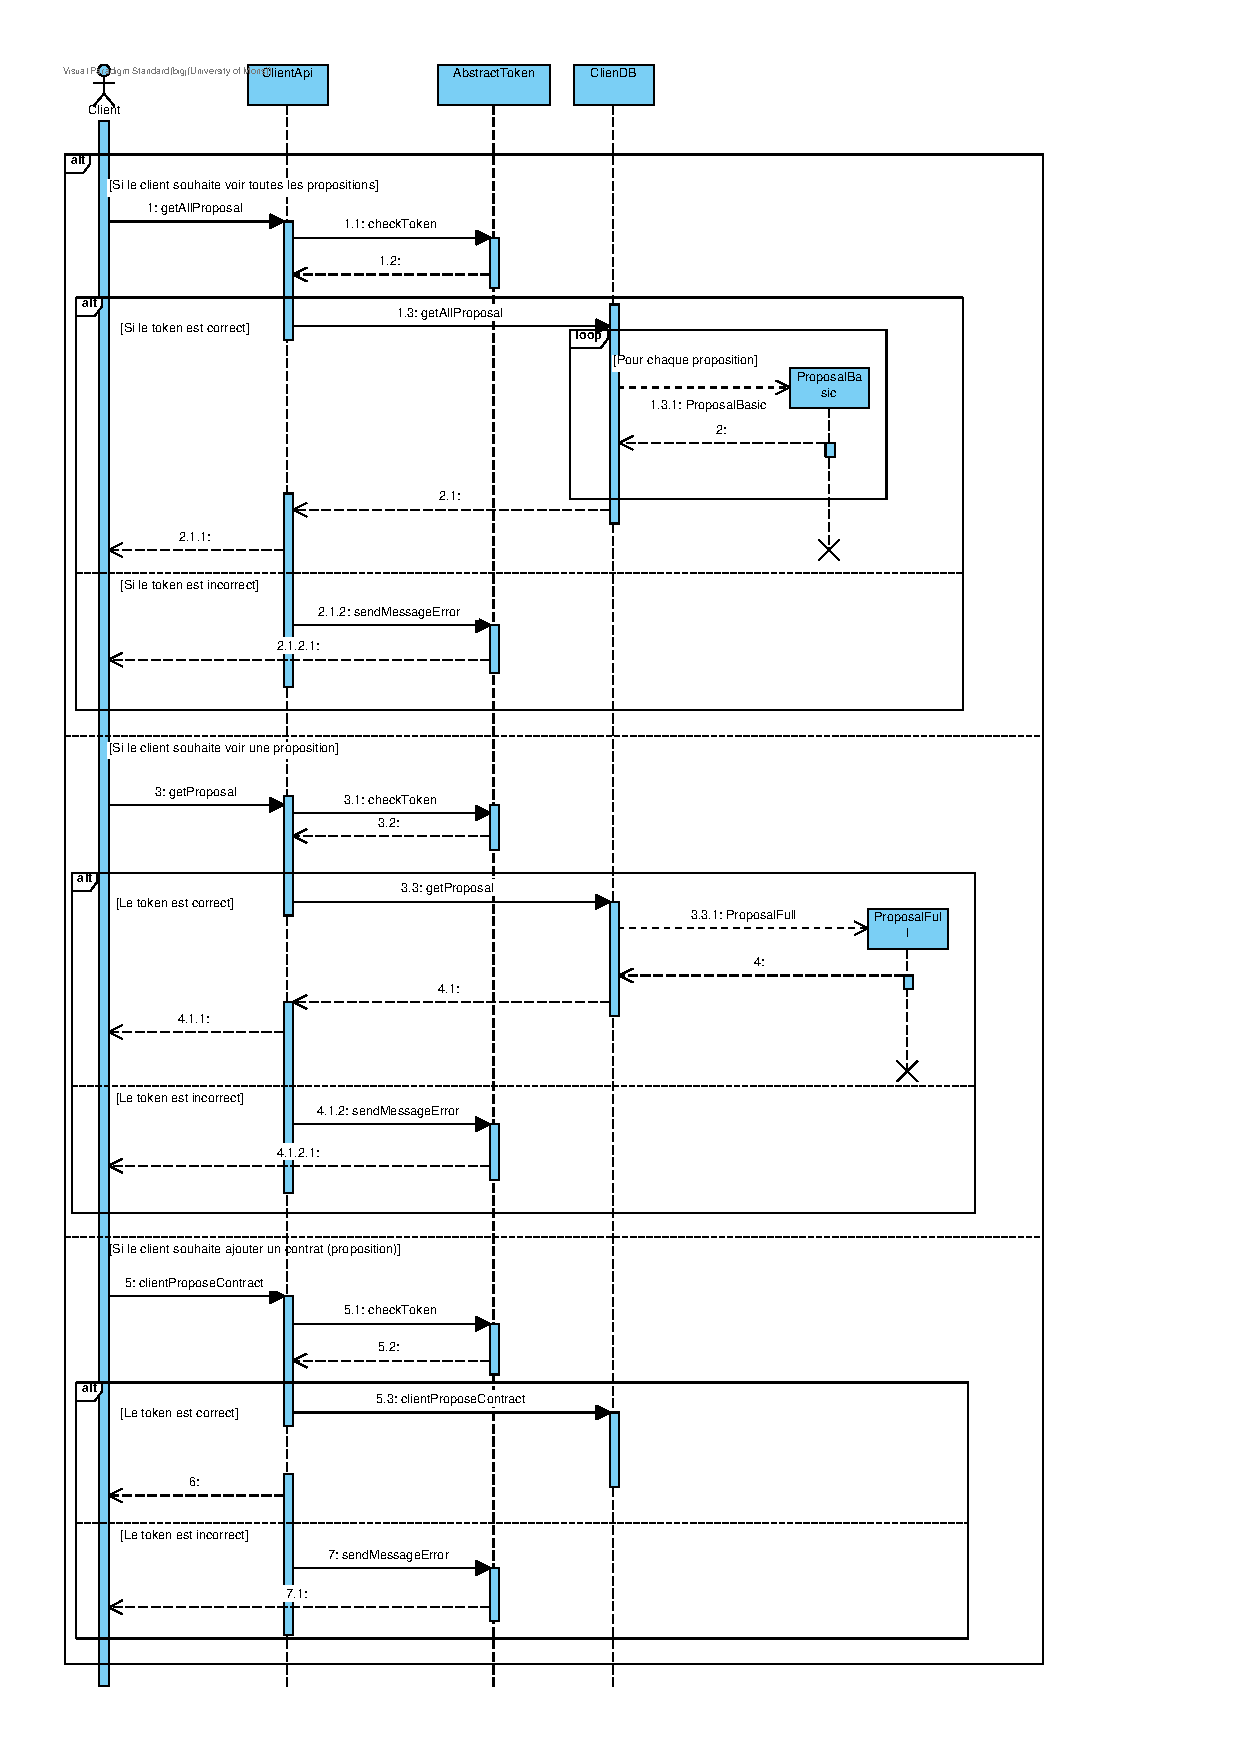
\includegraphics[height = 1.2\textwidth]{Base/sequence/img/client/seqFCRe.pdf}
\end{figure}

\newpage

\subsubsection{Portefeuilles}
\begin{flushleft}
L'Use case \textbf{"Voir les portefeuilles"} fonctionne de la même manière qu'expliqué précédemment pour "Voir les fournisseurs et contrats relatifs".
En effet, il y aura deux méthodes : 
\end{flushleft}
\begin{enumerate}
\item getAllWallet si le client souhaite voir tous les portefeuilles. On doit donc retourner une ArrayList de "walletBasic".
\item getWallet si le client souhaite voir un portefeuille en particulier. On doit donc retourner une instance de "walletFull".
\end{enumerate}

\begin{flushleft}
Passons maintenant aux Use Cases \textbf{"Créer un portefeuille"} et \textbf{"Fermer un portefeuille"}.
\end{flushleft}

\begin{flushleft}
Pour \textbf{créer un portefeuille}, nous appelons donc la méthode "createWallet" de clientApi et ensuite, la méthode du même nom de ClientDB.
\end{flushleft}

\begin{flushleft}
Nous créons une instance de "walletBasic", que nous devons enregistrer dans "ClientDB" avant de clôturer l'exécution de la méthode car il s'agit d'un nouveau portefeuille à stocker.
\end{flushleft}

\begin{flushleft}
Pour \textbf{supprimer un portefeuille}, nous appelons la méthode "deleteWallet" de clientApi.
\end{flushleft}
\begin{flushleft}
Cependant, avant d'appeler la méthode du même nom de ClientDB, nous devons vérifier que le portefeuille est vide.
\end{flushleft}
\begin{flushleft}
Si c'est le cas le portefeuille sera bien supprimé, sinon, on renverra une erreur.
\end{flushleft}

\newpage
\begin{figure}[h]
\centering
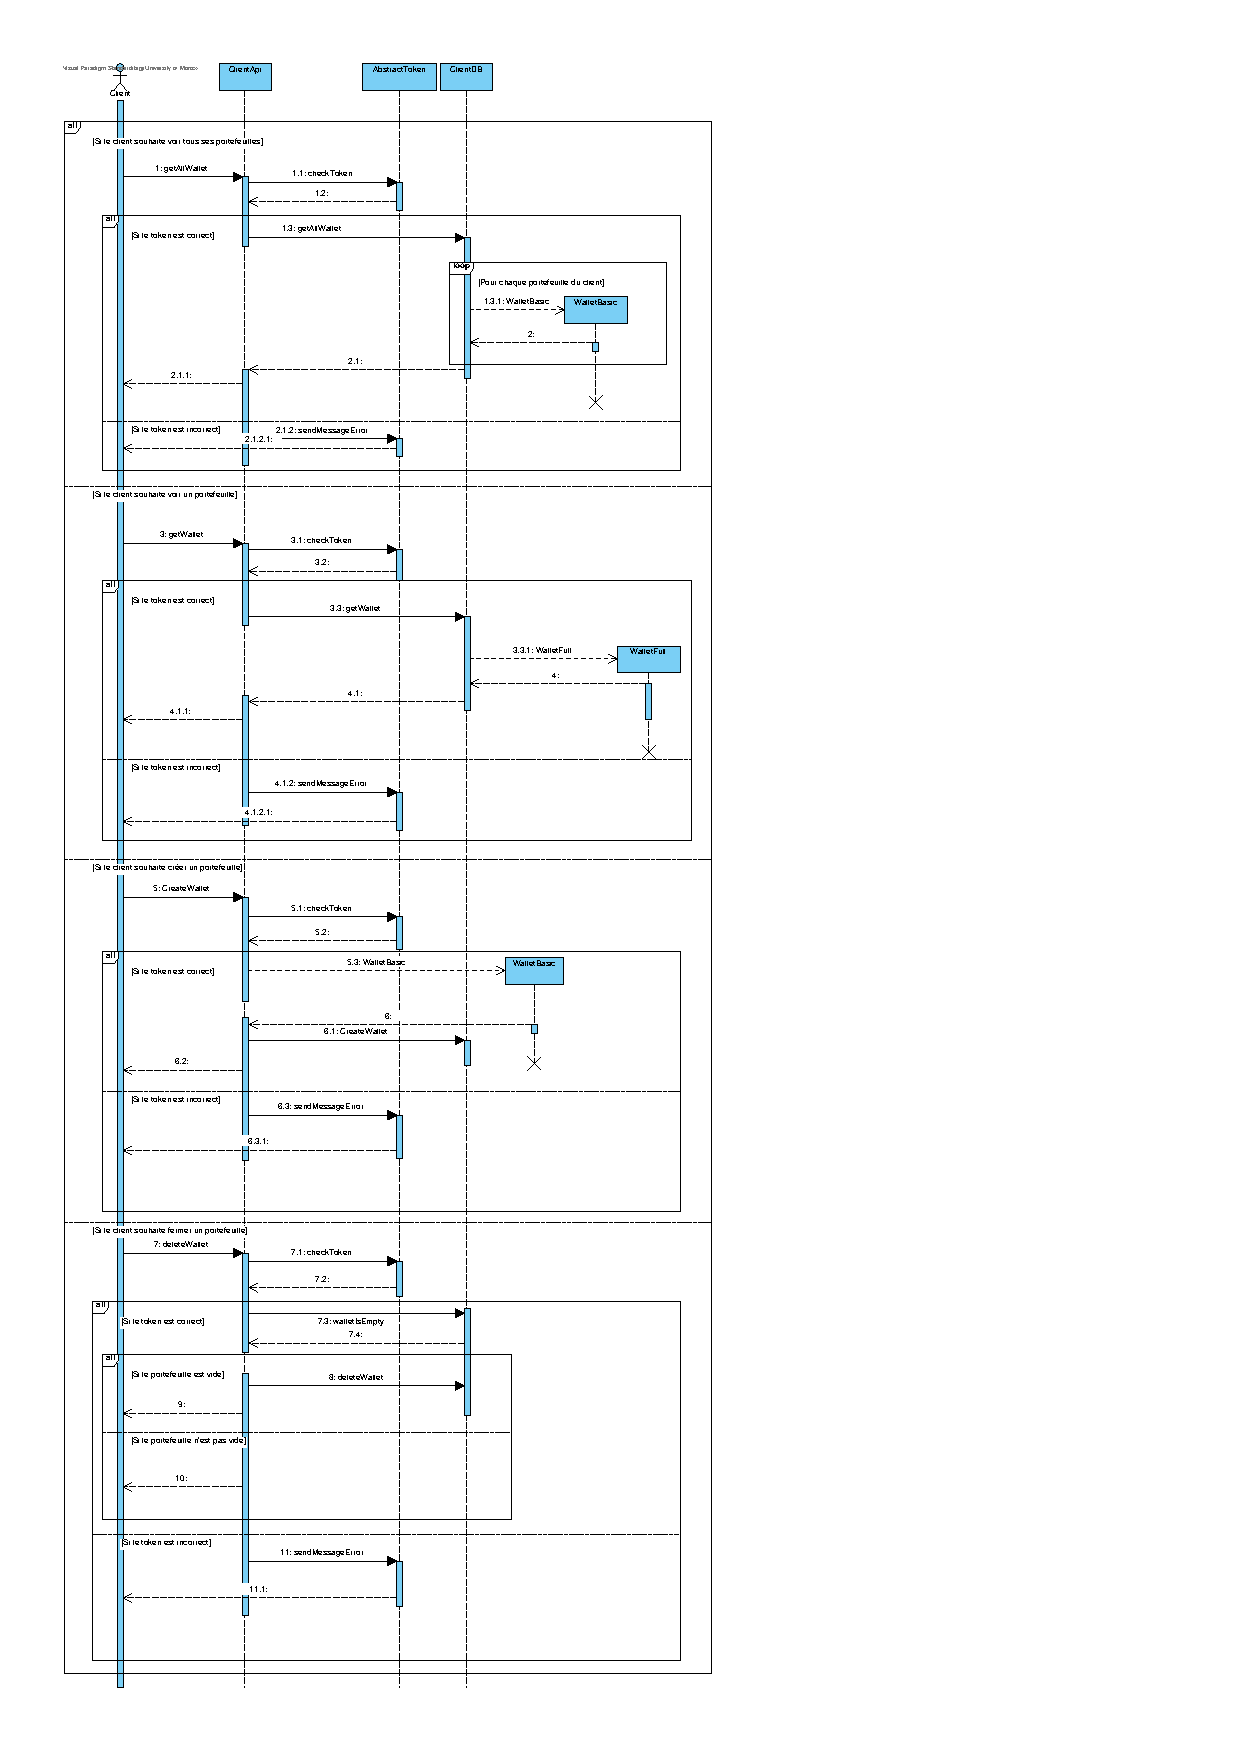
\includegraphics[height = 1.2\textwidth]{Base/sequence/img/client/seqPortefeuilles.pdf}
\end{figure}
\newpage

\subsection{Provider}

\begin{flushleft}
Tout d'abord, nous avons fait en sorte qu'un use case peut être représenté via un choix alternatif. Aussi, pour éviter de répéter la même chose dans le rapport, nous posons que toutes les méthodes liées à l'API appelleront la méthode \textbf{checkToken} de \textbf{AbstractToken} ce qui impliquera deux choix alternatifs : "Si le token est correct" et "Si le token est incorrect". Dans le dernier cas, on renverra un message d'erreur au fournisseur.
\end{flushleft}
\subsubsection{Gestion des clients}
\begin{flushleft}
Commençons par le use case "voir ses clients". Afin qu'un fournisseur puisse voir ses clients, il lui suffit d'appeler la méthode \textbf{getAllHisClients} dans la classe \textbf{ProviderApi} et \textbf{ProviderDB}. Etant donné qu'on retourne une collection d'objet \textbf{ClientBasic}. Nous devons utiliser une boucle. Pour voir un seul de ses clients, il lui suffit d'appeler la méthode \textbf{getClient}.
\end{flushleft}

\begin{flushleft}
Passons maintenant au use case "supprimer un client". Pour faire cela, la méthode \textbf{deleteClient} sera utilisée. Par conséquent, une notification sera envoyée au client ce qui nous oblige à faire appel à la méthode \textbf{createNotification}. 
\end{flushleft}

\begin{flushleft}
Pour ajouter un client, cela se fera par le biais d'une proposition du fournisseur au client. Ceci faisant appel à la méthode \textbf{providerProposeContract}. Nous posons comme hypothèse que le client n'a aucun contrat en cours avec le fournisseur. 
\end{flushleft}

\begin{flushleft}
Pour qu'un fournisseur puisse ajouter des clients. Il doit d'abord avoir accès à tous les clients de l'application. Ceci se fera par la méthode \textbf{getAllClients}. De la même manière que voir "ses clients", nous utiliserons une boucle.  
\end{flushleft}

\newpage
\begin{figure}[h]
    \centering
    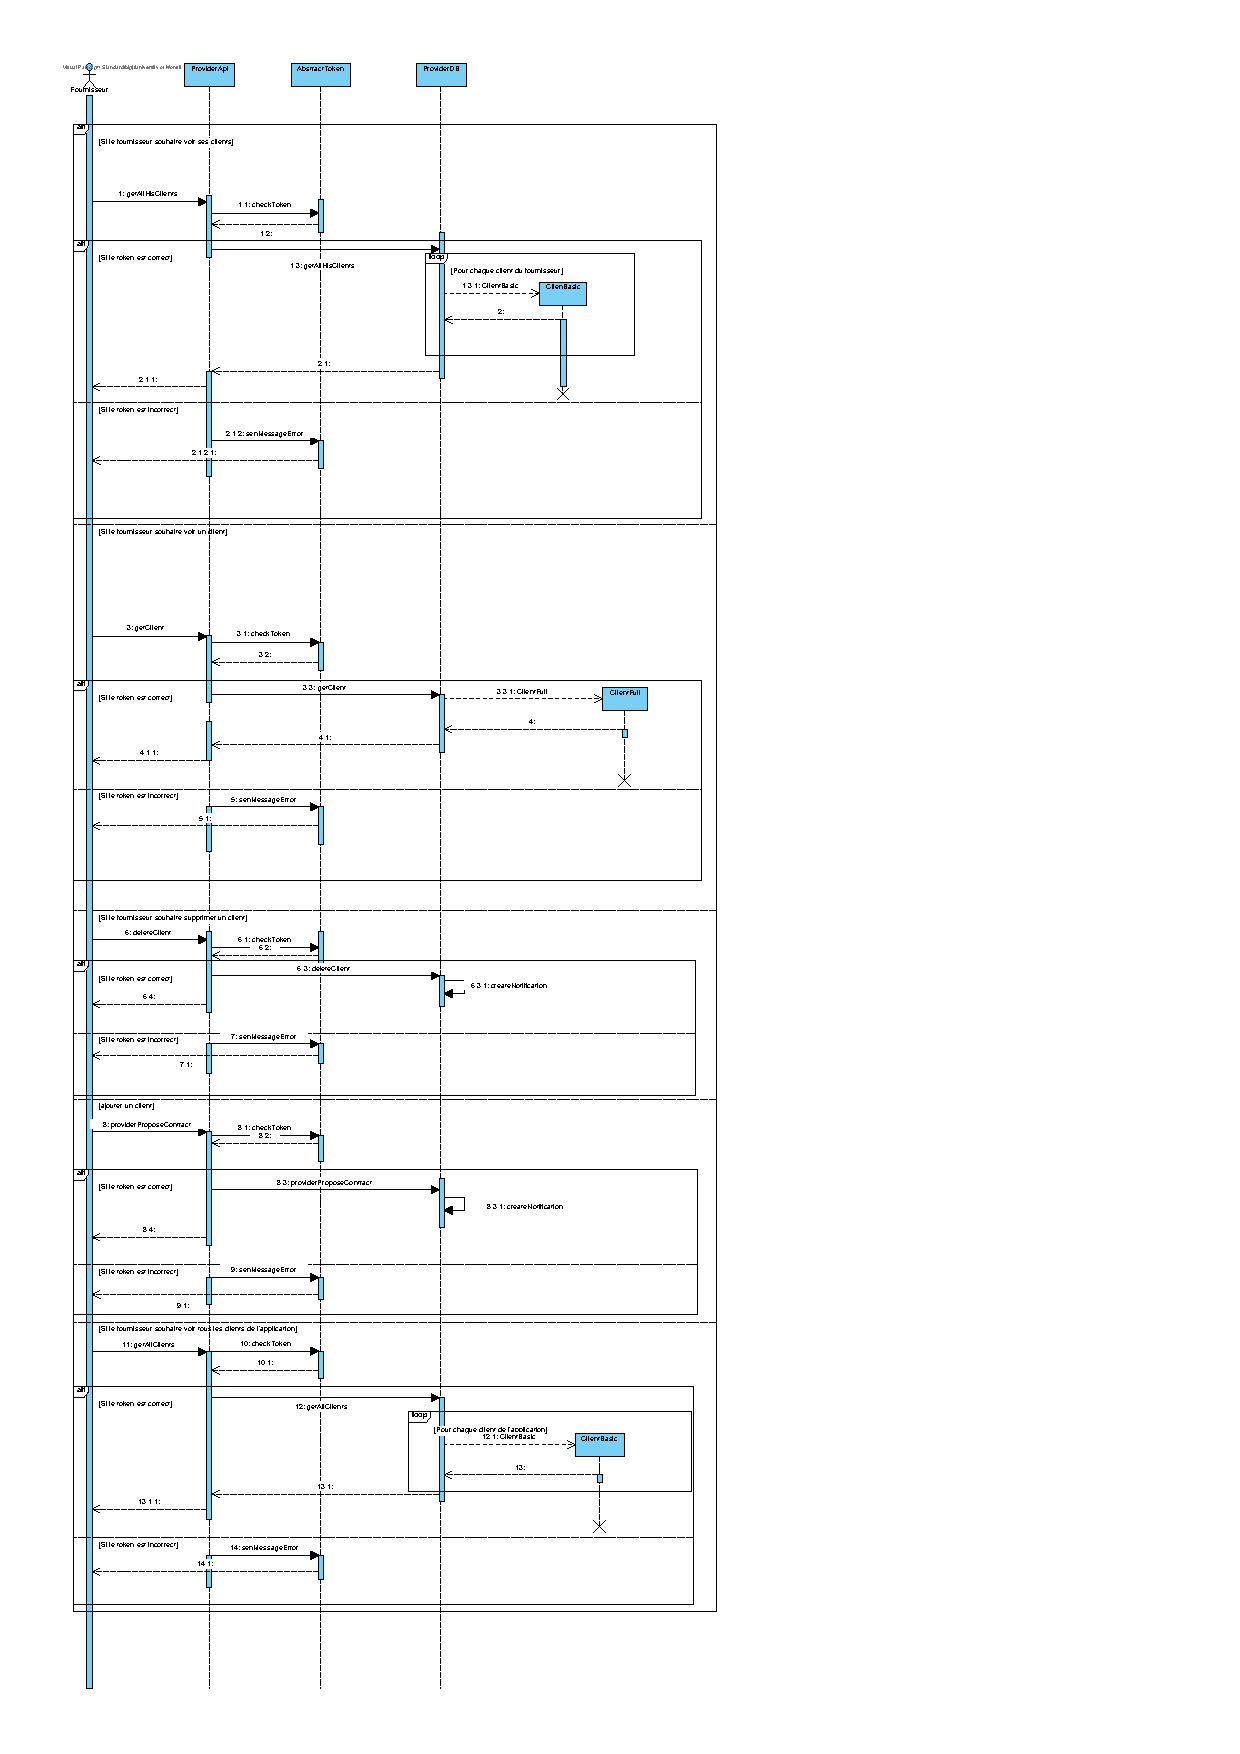
\includegraphics[height = 1\textwidth]{Base/sequence/img/fournisseur/voir_ses_clients.pdf}
\end{figure}
\newpage
\subsubsection{Gestion des propositions}
\begin{flushleft}
Avant de parler des diagrammes de séquence de cette partie. Nous avons choisi de mettre les contrats d'un fournisseur et ses propositions dans les use cases parlant des contrats. De plus, seules les propositions seront abordées dans cette partie étant donné qu'un contrat sera commun au fournisseur et au client(section \ref{CONTRATS},page \pageref{CONTRATS}).
\end{flushleft}

\begin{flushleft}
Pour commencer, nous allons regarder comment le fournisseur peut avoir accès à toutes ses propositions. Pour cela, il devra utiliser la méthode \textbf{getAllProposals}. De plus, une boucle permettra de récupérer tous les objets. Si le fournisseur veut avoir plus de précision sur une de ses propositions, alors il aura juste besoin d'apeller la méthode \textbf{getProposal} en ayant l'identifiant de la proposition au préalable.
\end{flushleft}
\begin{flushleft}
Après ça, Si le fournisseur veut ajouter une proposition. La méthode \textbf{addProposal} sera utilisée. Il faudra néanmoins créer un objet \textbf{ProposalFull} qui sera ensuite ajouté par la précédente méthode à la base de données. 
\end{flushleft}

\begin{flushleft}
Ensuite, si le fournisseur souhaite modifier les paramètres d'une de ses propositions. Il n'aura qu'à faire un nouvel objet qui servira de "remplacant" à l'ancienne proposition. La méthode \textbf{changeProposal} sera appelée par la suite pour faire le changement des paramètres directement dans la base de données. A noter que modifier les paramètres d'une proposition revient à changer les contrats avec les clients qui ont pris cette proposition. De ce fait, une notification sera envoyée via la méthode \textbf{createNotification}.
\end{flushleft}

\begin{flushleft}
Pour finir cette partie, nous allons parler de comment fonctionne la procédure pour supprimer une proposition. Nous avons juste à faire appel à la méthode \textbf{deleteProposal}. De manière similaire au fait de modifier, supprimer implique la supression des contrats des clients ayant comme base cette proposition ce qui implique l'envoi d'une notification par la méthode \textbf{createNotification}.
\end{flushleft}

\newpage
\begin{figure}[h]
    \centering
    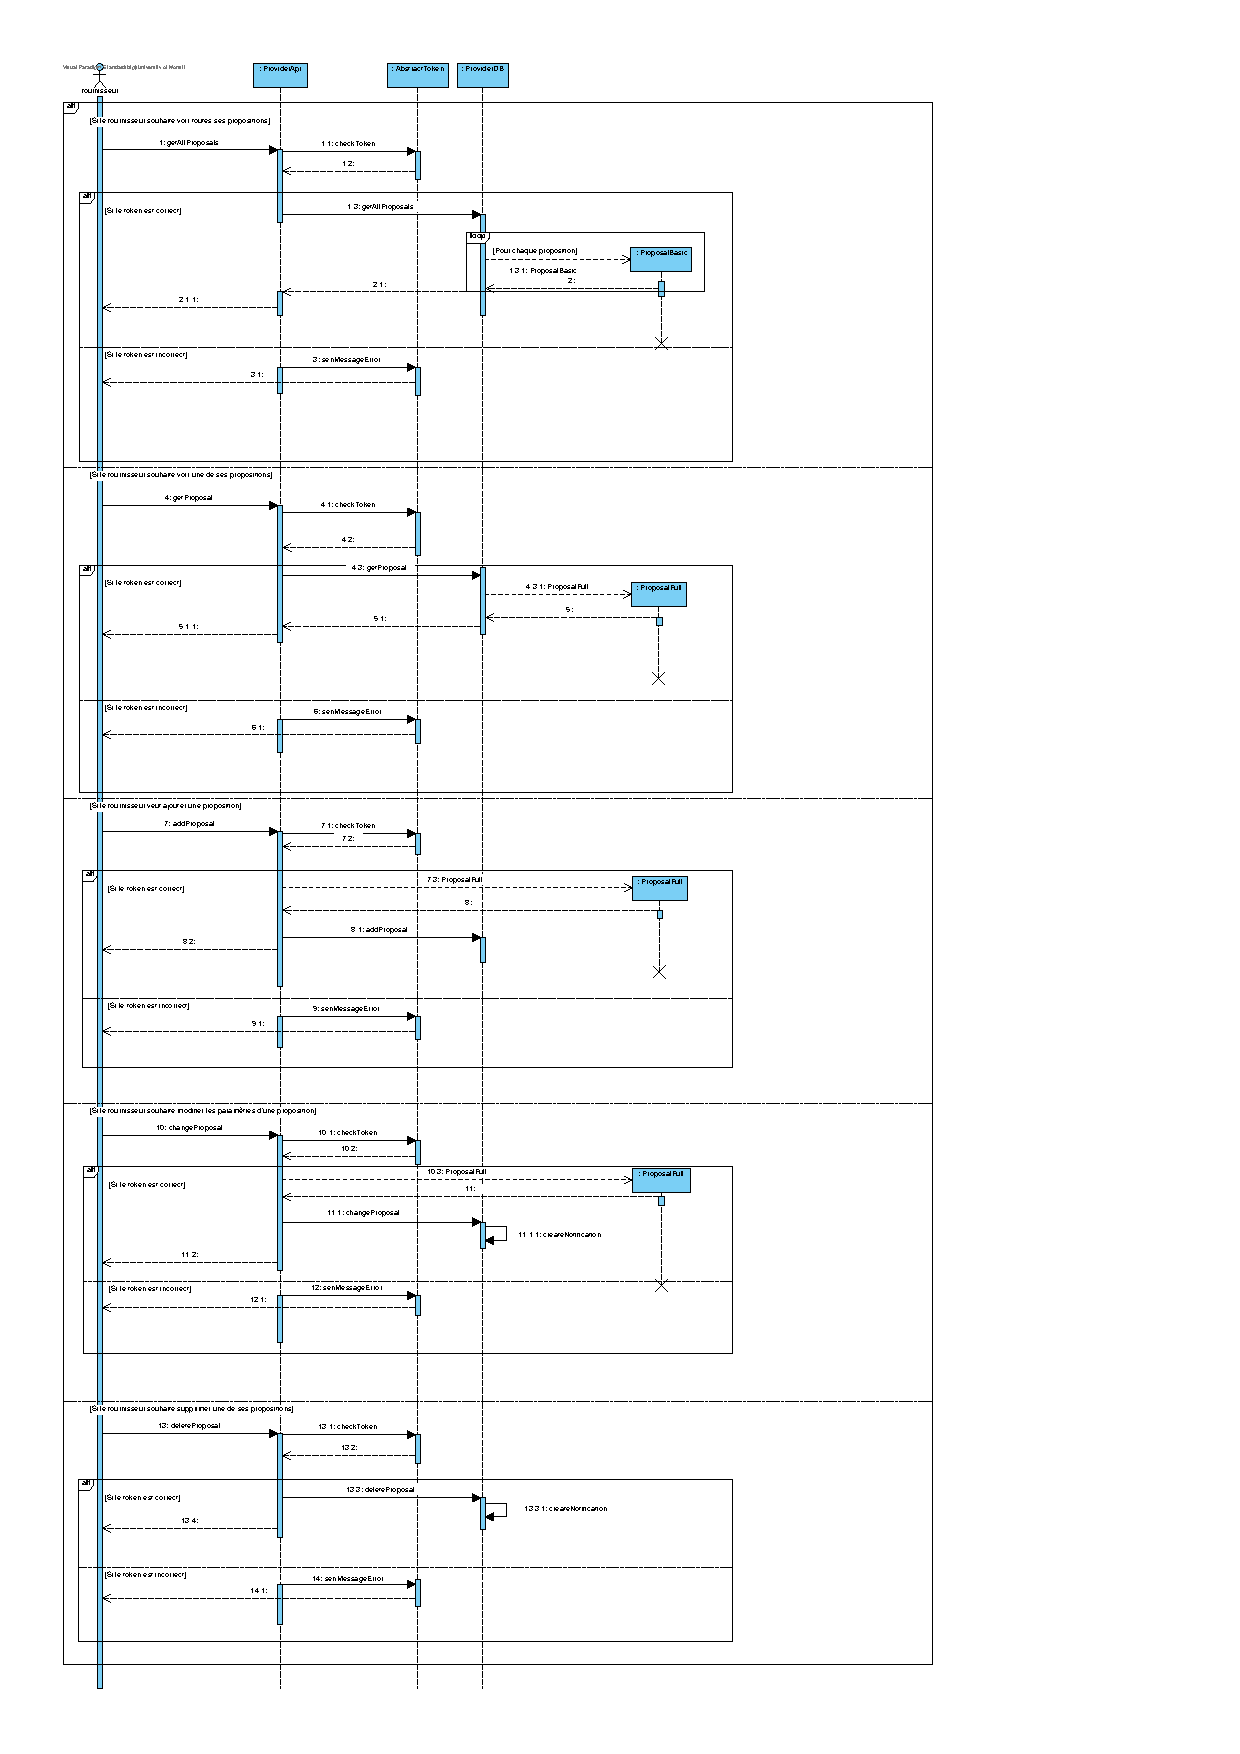
\includegraphics[height = 0.9\textwidth]{Base/sequence/img/fournisseur/voir_les_propositions.pdf}
\end{figure}

\newpage
\subsubsection{Gestion de la consommation}
\begin{flushleft}
Cette sous-sous-section parlera de la gestion de la consommation d'un client par le fournisseur. A noter que le fait pour un fournisseur de voir la consommation de ses clients est la même procédure qu'un client qui va voir ses consommations à l'exception qu'un fournisseur ne peut voir la consommation créée par le client liée à son contrat.     
\end{flushleft}

\begin{flushleft}
Tout d'abord, le fournisseur souhaitant supprimer une donnée de consommation devra passer par la méthode \textbf{deleteConsumption} de l'API. De plus, il aura besoin d'un objet date ne contenant que l'année, le mois et le jour. Après ça, il pourra supprimer la donnée qu'il souhaite avec la méthode portant le même nom que celle de l'API. Une notification sera envoyée au client avec la méthode \textbf{createNotification}.
\end{flushleft}

\begin{flushleft}
Ensuite, si le fournisseur souhaite supprimer toutes les données de consommation d'un client. Il aura juste besoin de la méthode \textbf{deleteAllConsumption}. De même que le paragraphe du dessus, une notification sera créée.
\end{flushleft}

\begin{figure}[h]
    \centering
    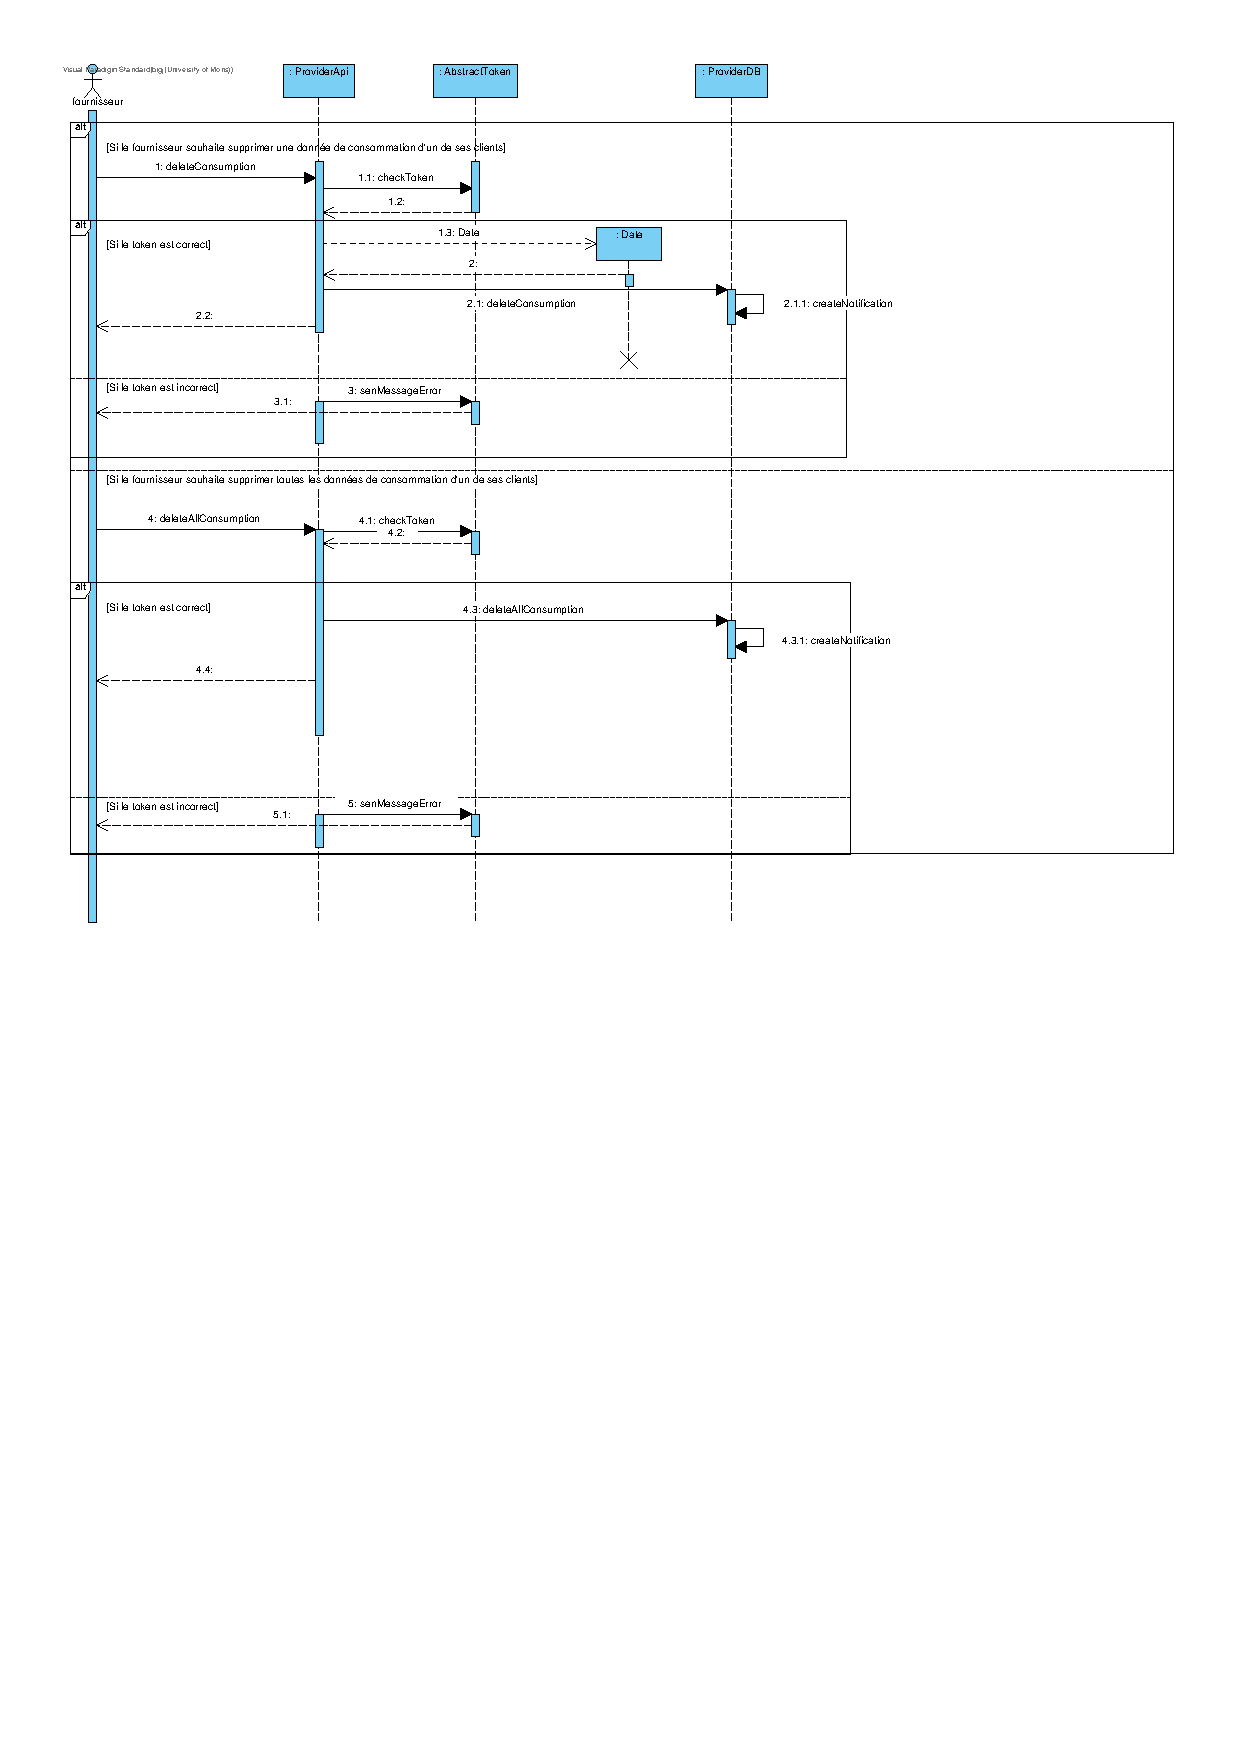
\includegraphics[height = 0.8\textwidth]{Base/sequence/img/fournisseur/gestion de la consommation.pdf}
\end{figure}
